\chapter{Guía de uso}

\section{Características del robot}
El simulador está programado para operar con una 
plataforma Gough-Cappel con los siguientes parámetros:

\begin{table}[htb!]
\centering
\begin{tabular}{lc}

\multicolumn{2}{c}{Parámetros de diseño} \\ \hline
Radio de la base ($r_b$) & $0.44205 \ [m]$ \\ 
Radio de la plataforma ($r_a$) & $0.36248 \ [m]$ \\ 
Separación entre juntas en la base ($k_b$) & $0.7 \ [m]$ \\ 
Separación entre juntas en la plataforma ($k_a$) & $0.2986 \ [m]$ \\ 
Longitud mínima del actuador ($q_{min}$) & $1.28929 \ [m]$ \\ 
Mangitud máxima del actuador ($q_{max}$) &  $2.19 \ [m]$ \\ 
\end{tabular}
\caption{Restricciones dimensionales del robot paralelo.}
\label{tab: restricciones}
\end{table}

\begin{figure}[htb!]
\centering
 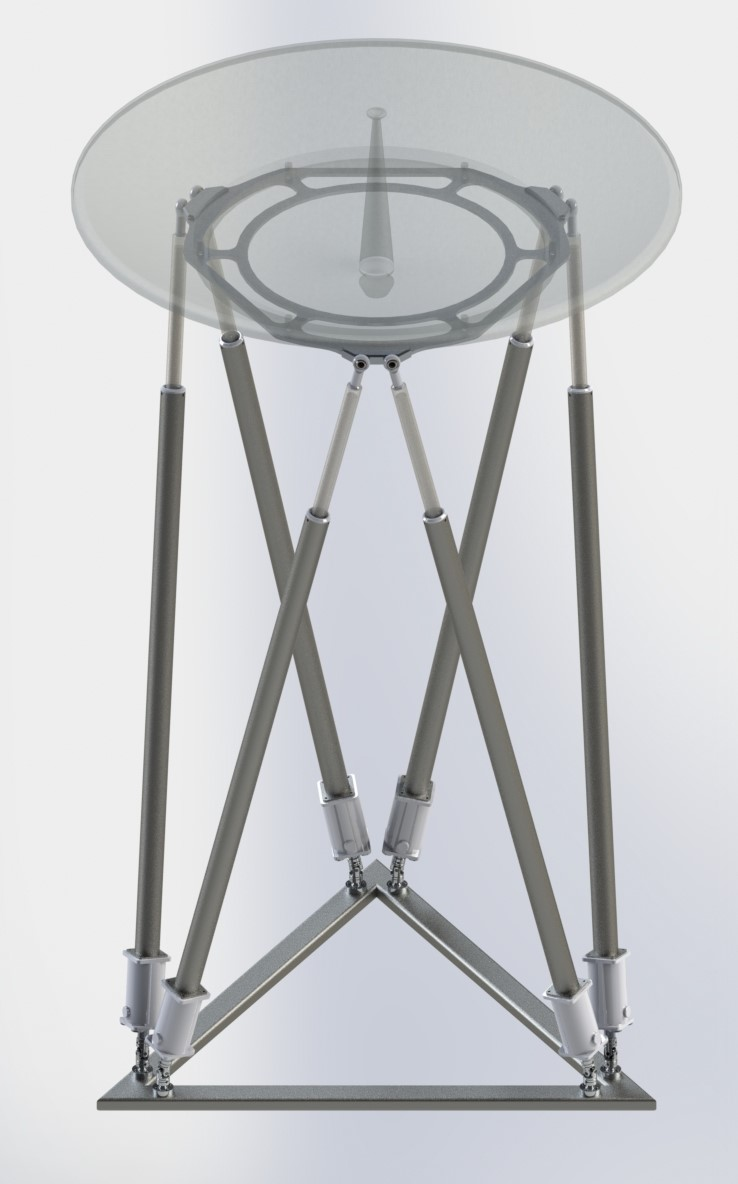
\includegraphics[scale=0.3]{PGScrop.jpg}
 \caption{Robot del simulador.}
\end{figure}


\section{Uso del simulador}
Se incluyen tres esquemas de control para simular el robot.
Estos archivos son llamados PGS\_PD, PGS\_PDpG y PGS\_PID respectivamente.
Cualquiera de estos esquemas puede ser empleado como plantilla
para la implementación de nuevas estrategias de control.

Para utilizar los esquemas es necesario abrir los archivos slx 
desde la interfaz de MATLAB.
También es importante agregar la carpeta de \textbf{funciones}
al \text{Path} de MATLAB 
(clic derecho en la carpeta y seleccionar Add to Path).

A continuación se presenta uno de los esquemas incluidos.

\begin{figure}[htb!]
\centering
 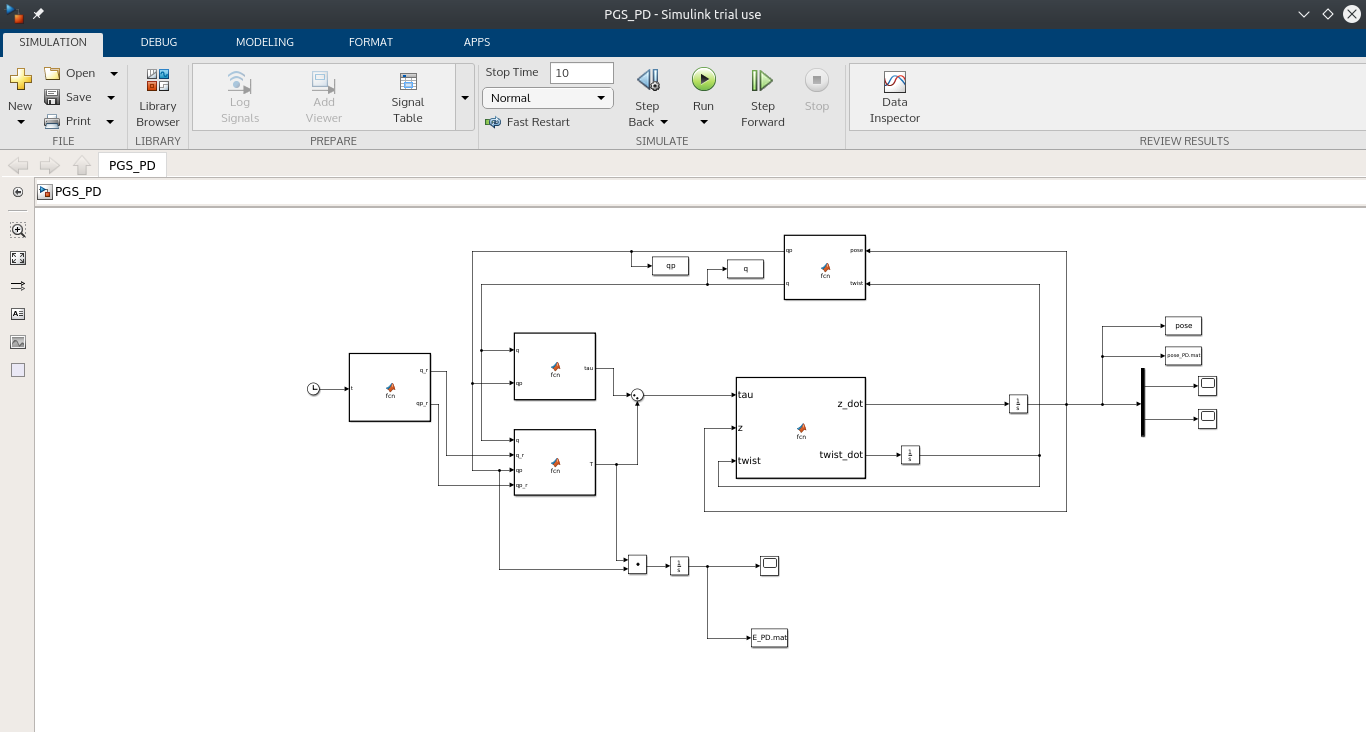
\includegraphics[scale=0.3]{PD.png}
 \caption{Esquema de control en SIMULINK.}
\end{figure}

Para iniciar la simulación es necesario 
presionar el botón de iniciar (Run) 
en la interfaz de SIMULINK.
El usuario es capaz de cambiar el tiempo de 
simulación desde la opción de Stop Time.

Una vez concluido el tiempo de simulación es 
posible observar los resultados con los 
Scopes incluidos en el programa.
Es posible observar la pose de la plataforma móvil
a través del tiempo y el cambio de las longitudes de los pistones.

\begin{figure}[htb!]
 \centering
 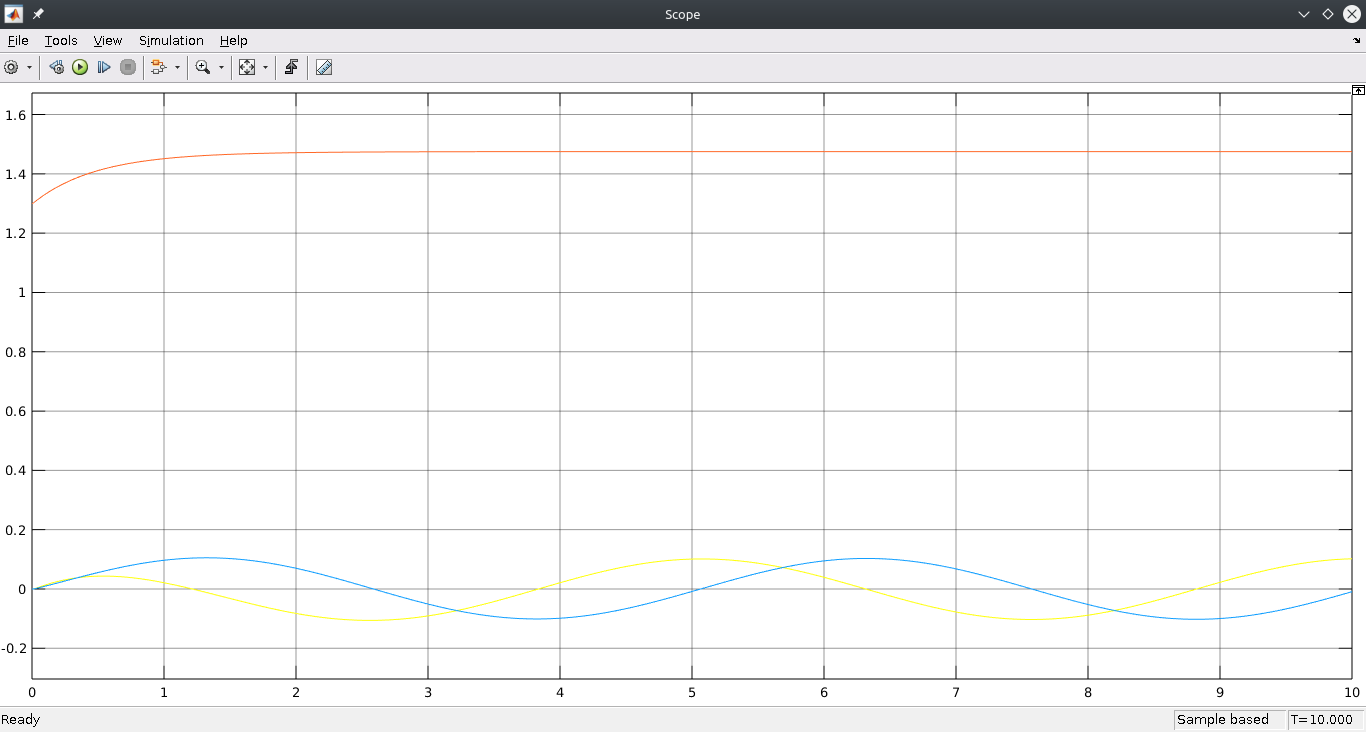
\includegraphics[scale=0.3]{plots.png}
 \caption{Resultados del simulador.}
\end{figure}



